\chapter{Thực nghiệm}
Với mục tiêu tìm hiểu và giải quyết bài toán phân loại thực khuẩn với dữ liệu đầu vào là contig, nhóm sinh viên thực hiện các thử nghiệm và đánh giá tương tự với nhóm tác giả DeePhage. Chương này trình bày phương pháp xây dựng bộ dữ liệu, các chỉ số đánh giá, kịch bản và kết quả thực nghiệm.

\section{Xây dựng bộ dữ liệu}
\subsection{ Xử lý nhãn }
Sau khi tìm hiểu các bài báo, nhóm sinh viên thực hiện xây dựng bộ dữ liệu mới dựa trên 2 bộ dữ liệu được sử dụng trong bài báo DeepPL và DeePhage. Nhãn $y$ của bản ghi $X$ được nhóm sinh viên xử lý như sau:
\begin{enumerate}
    \item Nếu $X \in DeePhage \Rightarrow y = y_{DeePhage}$ 
    \item Nếu $X \in DeepPL \Rightarrow y = y_{DeepPL}$
    \item Nếu $X \in DeePhage \cap DeepPL \Rightarrow y = y_{DeePhage}$
\end{enumerate}

\section{Kịch bản thực nghiệm}\label{ kịch bản thực nghiệm}
Để tiến hành các thực nghiệm, nhóm sinh viên chọn 2 mô hình là DeePhage và XGBoost. Nhận thấy DeePhage là công cụ  hài hòa trong nhóm các phương pháp dựa trên học sâu khi mà hiệu suất phân loại tốt đồng thời có thời gian huấn luyện nhanh, nhóm sinh viên quyết định chọn DeePhage là công cụ tiêu chuẩn trong các thực nghiệm. Ngoài ra, do cần 1 mô hình đủ mạnh để có thể có hiệu suất phân loại tốt cũng như nhanh trong quá trình huấn luyện, nhóm quyết định chọn XGBoost là mô hình được sử dụng để trực tiếp so sánh với DeePhage.

\section{Các chỉ số đánh giá}
Để đánh giá 1 cách toàn diện hiệu suất phân loại của mô hình chứ không chỉ tập trung vào nhãn 1, nhóm sinh viên sử dụng các chỉ số sau:
\begin{itemize}
    \item Accuracy: sử dụng để do lường hiệu suất phân loại chung của mô hình trên 2 nhãn.
    \item Sensitivity: sử dụng để đo lường dộ phủ của mô hình trên nhãn 1.
    \item Specificity: sử dụng để đo lường độ phủ của mô hình trên nhãn 0.
\end{itemize}


\section{Thực nghiệm với mô hình PHACTS}

\section{Thực nghiệm với mô hình Phage AI}
<<Nam điền kết quả>>

\section{Thực nghiệm với mô hình DeePhage}
<<Sơn điền kết quả>>

\section{So sánh kết quả thực nghiệm giữa các mô hình}


\subsection{So sánh hiệu suất phân loại giữa DeePhage và XGBoost trên bộ dữ liệu xây dựng}

\begin{figure}[H]
    \centering
    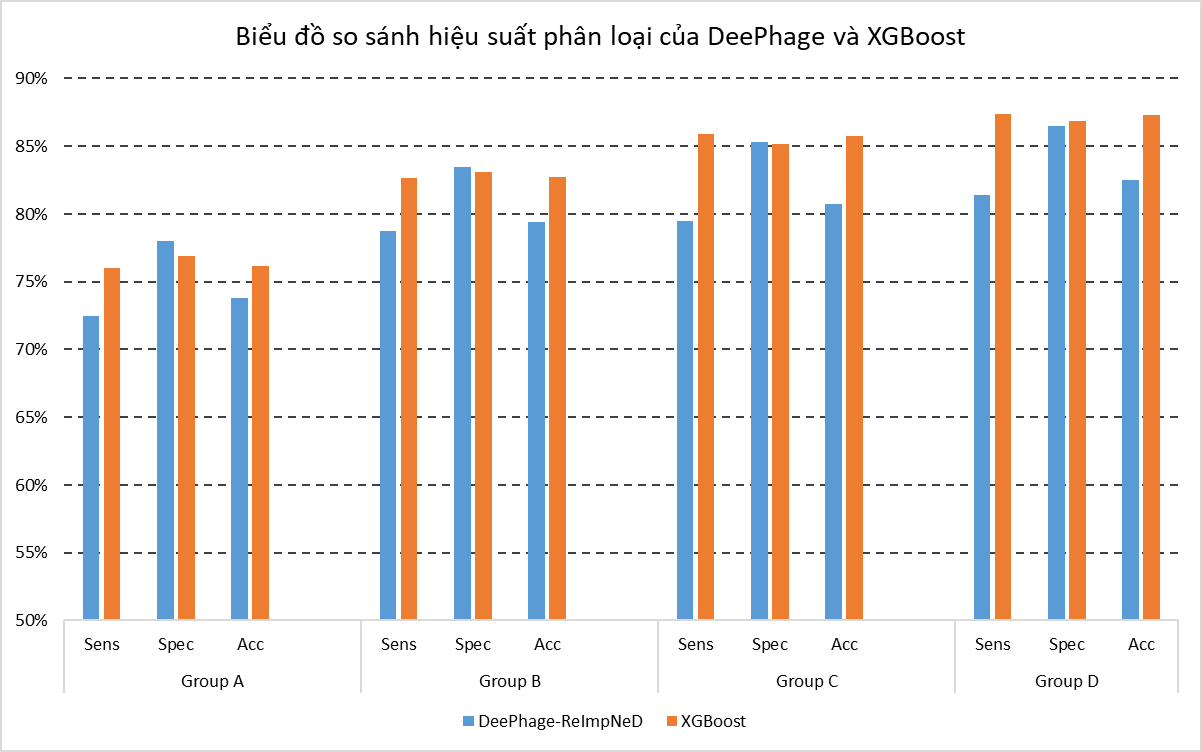
\includegraphics[width=1\linewidth]{figures/result_deephage_vs_xgboost.png}
    \caption{Kết quả hiệu suất phân loại của mô hình XGBoost trên tập dữ liệu xây dựng.}
    \label{fig:result_2}
\end{figure}

Hình \ref{fig:result_2} là biểu đồ so sánh hiệu suất phân loại của DeePhage và XGBoost trên tập dữ liệu mà nhóm sinh viên xây dựng. Có thể thấy, DeePhage cho kết quả tốt hơn 1 chút, khoảng từ 2\% - 5\% khi hơn XGBoost ở 2 chỉ số Sensitivity và Accuracy. Nghĩa là DeePhage cho khả năng nhận diện nhãn 1 và độ chính xác tổng thể cao hơn. Với chỉ số Specificity, XGBoost cho kết quả tốt hơn khoảng 5\%, nghĩa là khả năng nhận diễn nhãn 0 của XGBoost tốt hơn DeePhage.

